\documentclass[a4paper,12pt,twoside,openright]{report}
\usepackage[english]{babel}
\usepackage{graphicx}
\usepackage{csvsimple}
\usepackage{pgfplotstable}
\usepackage{booktabs}
\usepackage{chngcntr}
\usepackage{sectsty}
\usepackage{pdfpages}
\usepackage{longtable}
\usepackage{tocloft}
\usepackage{amsmath}
\usepackage{amsfonts}

%\usepackage[pdftex]{graphicx}
\usepackage[utf8]{inputenc}
\DeclareUnicodeCharacter{2010}{-}
\usepackage{geometry}
%\usepackage{bbold}
\geometry{a4paper,left=2.5cm,right=2.5cm, top=2.5cm, bottom=3cm}
\newcommand{\HRule}{\rule{\linewidth}{0.5mm}}

\usepackage{textcomp}
\usepackage[hyphens,spaces]{url}
\usepackage{setspace}

\usepackage[author={Julian Schmidt}]{pdfcomment}

\setcounter{topnumber}{2}
\setcounter{bottomnumber}{2}
\setcounter{totalnumber}{4}
\renewcommand{\topfraction}{0.85}
\renewcommand{\bottomfraction}{0.85}
\renewcommand{\textfraction}{0.15}
\renewcommand{\floatpagefraction}{0.7}

\begin{document}
\sloppy
\chapterfont{\LARGE}
\sectionfont{\Large}
\subsectionfont{\Large}
\subsubsectionfont{\Large}
\counterwithin{figure}{chapter}
\counterwithin{table}{chapter}

\begin{titlepage}


%%LR
\sffamily

\begin{center}


% Oberer Teil der Titelseite:

\includegraphics[width=0.3\textwidth]{../figures/LMU-logo.jpg}
\hfill

\includegraphics[width=0.4\textwidth]{../figures/TUM-logo.jpg}  
\\[5cm]

{\LARGE Department of Bioinformatics and Computational Biology}\\[0.5cm]
{Technische Universit\"at M\"unchen}\\
[2cm]
{\Large Master's Thesis in Bioinformatics}\\[1.5cm]

% Title
\HRule \\[0.4cm]
\begin{spacing}{1.6}
{\huge \bfseries Variation of HERV elements in the KORA cohort
}
\end{spacing}
\HRule \\[1.5cm]

{\Large Julian Schmidt}\\[2.5cm]

\vfill
\end{center}
\end{titlepage}
\pagestyle{empty}

%%LR comprehensive title
\begin{titlepage}
{\sffamily


\begin{center}

\includegraphics[width=0.3\textwidth]{../figures/LMU-logo.jpg}
\hfill

\includegraphics[width=0.4\textwidth]{../figures/TUM-logo.jpg}  
\\[1.5cm]  

{\LARGE Department of Bioinformatics and Computational Biology}\\[0.5cm]
{Technische Universit\"at M\"unchen}\\[1cm]
\begin{spacing}{1.6}
{\Large Master's Thesis in Bioinformatics}\\[1.6cm]
{\textbf{\LARGE Variation of HERV elements in the KORA cohort}}\\[1.6cm]
{\textbf{\LARGE Variation von HERV elementen in der KORA Kohorte}}\\[3.6cm]
\end{spacing}

\end{center}
\begin{center}\Large
  \begin{tabular}{ll}
    Author:& Julian Schmidt\\
    Supervisor: & Dr. Matthias Heinig\\
    Advisor:        & Johann Hawe\\
    Submitted:     &  15.04.2018\\
  \end{tabular}
\end{center}

}% end title page
\end{titlepage}


\vspace*{6cm}
\begin{center}
\begin{minipage}{.6\textwidth}
I confirm that this master's thesis is my own work and I have documented all sources and material used.
\\[2cm]
\begin{tabular}{p{0.3\textwidth} p{0.7\textwidth}}
13.04.2018 & \hrulefill \\
& \hspace{1.95cm} Julian Schmidt
\end{tabular}
\end{minipage}
\end{center}

\newpage

\pagenumbering{gobble}

\tableofcontents
\newpage

\pagestyle{plain}
\pagenumbering{arabic}
\chapter{Introduction} 
\label{Introduction}

\section{Human endogenous retroviruses}
\label{Introduction:Human endogenous retroviruses}

When the draft for the first human genome was published in 2001\cite{Venter1304} it was expected, that it would allow to fully understand the human genome. But soon after genes were annotated less than 5\% of the genome was found to be protein coding\cite{Consortium2001} and later on the amount of exonic protein coding DNA was estimated to be as low as 1.2\%\cite{Encode2012}. The remaining majority of the genome was often labeled as non-functional "junk DNA"\cite{Pennisi1159}. 

Since then this notion has generally been revoked. Especially within the two phases of the Encyclopedia of DNA Elements (ENCODE) project\cite{Encode2012}, participation in some functional role has been assigned to up 80.4\% of the human genome. 

%TODO write fitting segue
Still up to this day there are areas in the genome that are difficult to analyze. Especially repetitive sequences cause huge problems for any method that relies on sequencing\cite{Treangen2011}. In human repetitive DNA makes up about 50\% of the whole Genome\cite{Treangen2011}. There are five major classes of repetitive elements: Satellites, short interspersed nuclear elements (SINE), long interspersed nuclear elements (LINE), DNA transposons and long terminal repeat (LTR) retrotransposons. 

%TODO go deeper into retrotransposons
In this work we will focus on a subclass of the latter repeat class. Human endogenous retroviruses (HERVs) belong to the class of LTR retrotransposons and make up about 8\% of the human genome\cite{APM:APM12476}. HERVs originate from retroviruses that infected the germ line of humans or human ancestors up to 30 million years ago\cite{10.1146/annurev.genom.7.080505.115700}. Therefore, they became dormant in the genome and are inherited in a Mendelian fashion. Newly integrated endogenous retroviruses (ERVs) share the typical structure of the viruses they originate from. This means they contain at least the four main genes in the order $5'-gag-pro-pol-env-3'$. Gag encodes the matrix and capsid proteins. Pro codes for a protease. Pol is the reverse transcriptase and integrase and env codes for the surface proteins. Furthermore, they have two flanking LTRs that originate from a duplication of the sequence, where the retrovirus was integrated\cite{10.1146/annurev.genom.7.080505.115700}. An example of the structure of a HERV element is shown in figure \ref{fig:herv.structure.example}.

\begin{figure}[tb]
	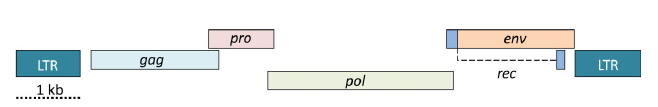
\includegraphics[scale = 0.92, keepaspectratio = true]{../figures/herv_structure_example}  
	\caption{Exemplified structure of an intact HERV element. Based on a HERV-K provirus, which is considered the most recently introduced in humans and contains the most complete viral genes. Taken from Young et. al. \cite{BIES:BIES201300049}}
    \label{fig:herv.structure.example}
\end{figure}

However, endogenous retroviruses in human are generally not able to replicate. This is due to a high level of degeneration of the HERV gene sequences due to mutations and deletions introducing frame shifts and premature stop codons. Homologous recombination of the flanking LTRs can also lead to elements containing only a single LTR and losing the entire coding body\cite{10.1146/annurev.genom.7.080505.115700}. Additionally, the promoter activity of LTRs is commonly silenced by hypermethylation\cite{Smith2013}.

Regardless of their loss of capability to replicate there still are multiple ways in which HERVs can influence human cells. LTRs of HERVs can act as promoters or enhancers to regulate gene expression. This has been associated to various cancers\cite{10.3892/ijmm.2013.1460}. While most HERV genes are degenerated, some are still expressed. A change in the transcription of several HERV subclasses was found in schizophrenia subjects, but the mechanisms of HERV involvement are not yet well understood\cite{10.3389/fpsyt.2015.00183}. Finally, non-coding HERV RNAs have been found to play a role in control of stem cell properties\cite{APM:APM12476}. 

\section{Multiomics}
\label{Introduction:Multiomics}
The rise of high-throughput technologies allows researchers to paint a more complete picture of the mechanisms of cell processes than ever before. Multi-omics, the combination of the analysis of different types of cellular molecules, is made possible by that. The objective of multi-omics studies is to draw conclusions about cellular mechanisms and understand the flow of information by finding associations and patterns connecting them\cite{Hasin2017}. In this work we worked on data from the fields of transcriptomics, genomics and epigenomics to investigate the effects of changes in human endogenous retroviruses (HERVs), which are introduced in more detail in section \ref{Introduction:Human endogenous retroviruses}.

Transcriptomics examines the occurrence and level of RNAs on a genome-wide scale. Following the central dogma of molecular biology, RNA is the intermediate between DNA and proteins and therefore of central importance\cite{}. With the late progress in transcriptome studies, even more effects of RNA have been discovered in the form of several functional RNAs\cite{10.3389/fgene.2015.00002}. RNA levels can be measured using a technology called RNA-seq\cite{Wang2009} or probe-based arrays\cite{Schulze2001}, as was the case with the data used in this work. 

The second field, genomics, describes variation between genomes. In this work we focused on single nucleotide polymorphisms (SNPs), which are single base changes. Genotypic information fills a special place in multi-omics analyses, as it not dependent on the environment and can be considered static in ones lifetime. Therefore, it is considered as the cause of changes instead of being a downstream effect of other changes\cite{Hasin2017}. This means they are an exceptional anchor for the start of multi-omics analyses. 
Genotypic changes are known to cause Mendelian diseases, when the change lies in the coding region of a protein. They also influence gene expression levels, which in turn is thought to be the cause of common diseases\cite{Hasin2017}.

Epigenomics is the youngest field of 'omics' that is used in this work. It describes genome-wide reversible modifications of DNA and DNA-associated proteins. Among these are multiple different histone modifications and DNA methylation. Epigenetic modifications play a major role in the regulation of gene transcription\cite{Piuntiaad9780,Deaton2011} and in general are a additional layer of information on top of the DNA sequence. Changes in epigenetic modifications are influenced by genetic and environmental factors\cite{Hasin2017}.

DNA methylation, the modification that is the focus in this work, is the best understood and researched epigenetic mark\cite{Smith2013}. The term refers to the addition of a methyl group to the fifth carbon atom of a cytosine ring, thus transforming the cytosine to 5-methylcytosine. In humans this happens almost exclusively in the context of a cytosine neighbored by a guanine - a CpG-site. As the complementary sequence of CG is also CG, methylation usually occurs on both strands. 

There are about 28 million CpG sites in the human genome, of which 60-80\% are generally methylated\cite{Smith2013}. The distribution of CpGs can be divided into two modes: The majority of the genome is sparsely populated by CpGs, that are usually methylated. Second, there are CG-dense regions, which are predominantly nonmethylated. These are called CpG islands and occur mainly around the transcription start sites of genes\cite{Deaton2011}. The methylation of these CpG islands is strongly connected to the silencing of adjacent genes, by preventing the transcription initiation\cite{Deaton2011}. Other mechanisms that are negatively affected by DNA methylation are general promoter, enhancer and insulator activity as well as transcription factor binding\cite{Smith2013}. 

%DNA methylation in humans is controlled by three enzymes called DNA methyl transferase  1 (DNMT1), DNMT3A and DNMT3B\cite{Smith2013}.
%TODO add placenta fusion effect of HERVs, exchange finally again

The multiomics data analyses performed in this work were either started from an anchor relating to HERV elements or performed genome wide and afterwards filtered to retain HERV specific results. 

\section{Effect network analysis}
\label{Introduction:Effect network analysis}
Many multiomics analyses are based on the calculation of associations within or between different data layers. Examples are co-expression of genes or the association of genotypic variants and transcription,  protein or methylation levels. These approaches allow to identify associated entities by calculating correlations between single entities over available individuals or samples. They can't give any resolution on the direction of an effect. Furthermore, purely correlation based methods can not differentiate between direct and indirect effects\cite{Hasin2017}.

Multomics data can be organized into networks, where each entity from the different layers is a node and the significant pairwise associations, that exceed a given threshold,  are resembled by undirected edges. However when using Pearson correlation as measurement of association, the networks tend to be rather dense, as indirect associations are still contained\cite{Krumsiek2011}. 

An approach to remove these indirect associations is the use of partial correlation coefficients. The partial correlation coefficient can be seen as the pairwise correlation between two variables conditioned against their correlations with all other variables. A scheme of how partial correlations work is shown in figure \ref{fig:partial.correlation.scheme}.

An approach that combines partial correlation coefficients with Bayesian structure learning is called "Gaussian Graphical Models"\cite{Krumsiek2011} (GGMs). We used GGMs to investigate the mechanisms of cellular control related to variation within HERV elements.

The Gaussian Graphical Models used in this work are described in more detail in section \ref{Methods:Gaussian Graphical Models}.

\newpage
\chapter{Data}
\label{Data}

\section{HERV annotation}
\label{Data:HERV annotation}
As mentioned in section \ref{Introduction:Human endogenous retroviruses} HERV elements tend to be highly degenerated. Therefore, it is no trivial task to pertain a complete HERV annotation for the human genome. Furthermore, classification and naming of endogenous retroviruses is not performed in an unified manner but rather dependent on how and by whom a given element was identified. 
Instead of collecting a library of known HERV sequences and performing sequence search ourselves, HERV annotations were pertained from RepeatMasker\cite{RepeatMasker} repeat library. RepeatMasker is a tool that screens DNA sequences against a library interspersed repeats and low complexity DNA sequences. It generates an annotation of identified repeats and masks them in the query sequence.

The track representing all identified repeats from the RepeatMasker library for human genome hg19 was downloaded from the UCSC genome browser download section \url{(http://hgdownload.soe.ucsc.edu/goldenPath/hg19/database/rmsk.txt.gz)}. It contains a total of 5298130 occurrences of repeats. Each entry consists of 17 values. These are repeat name, the repeat class and family, as well as the chromosome, strand, and the genomic start and end position of the repeat occurrence. Furthermore it contains the area of the known repeat sequence, that is covered by the occurrence. It also contains the quality of the alignment of the repeat sequence to the annotated position using the Smith Waterman alignment score\cite{SMITH1981195} and the number of base mismatches, deletions and insertions per thousand base pairs. Finally, there is an indexing field used to speed up chromosome range queries and the first digit of the id field in the RepeatMasker output file. The first 10 lines of the track are shown in table \ref{tab:RepeatMaskerTrack}.

\begin{table}[b]
\centering
\label{tab:RepeatMaskerTrack}
\resizebox{\textwidth}{!}{
\pgfplotstabletypeset[
    col sep=tab, 
    header=true,    
	columns={bin, swScore, milliDiv, milliDel, milliIns, genoName, genoStart, genoEnd, genoLeft, strand, repName, repClass, repFamily, repStart, repEnd, repLeft, id},
	columns/genoName/.style={column type=l,string type},
	columns/strand/.style={column type=l,string type},
	columns/repName/.style={column type=l,string type, string replace*={_}{\textunderscore}},
	columns/repClass/.style={column type=l,string type, string replace*={_}{\textunderscore}},
	columns/repFamily/.style={column type=l,string type, string replace*={_}{\textunderscore}},
	every head row/.style={before row=\hline, after row=\hline},
	every last row/.style={after row=\hline}]{../tables/head.repeatmasker.track.tsv}}
\caption{First ten rows of the RepeatMasker annotation on hg19}
\end{table}

To extract HERV elements the annotation was filtered on different columns generating three sets of variable size. Multiple HERV sets were created as an attempt to cover different possible definitions of HERV elements.

This work only discerned between different HERV element types by defining different HERV sets. Therefore, within each set annotations, whose genomic positions overlap or are directly adjacent, were merged into one element.

A first set, HERV set 1 (HERV S1) was constructed by extracting all elements that contained "ERV" in the repeat name column. This set
The resulting 42508 annotations condensed to 35358 elements after merging. The elements have a mean width of 956 bp and cover a total of 33.8 Mbp, which is about 1.04\% of the human genome.  

Alternatively, filtering the annotation for "ERV" in the super family column leads to 696689 annotations. HERV set 2 (HERV S2) contains all endogenous retroviral sequences found in the human genome. Therefore, it is the most comprehensive set and it is the focus of detailed results that are shown and discussed. After merging overlapping and adjacent annotations this led to 612594 elements. Their mean width is 430 bp and they make up to 263.4 Mbp or ca 8.13\% of the human genome. The distribution of element lengths in HERV S2 is shown in Figure \ref{fig:hervS2.length.hist} 

A third set "HERV set 3" (HERV S3) was constructed by filtering the repeat name column for "HERV", which resulted in 21361 annotations. As this set contains only elements that are explicitly named "HERV", we expect it to contain elements, that were inserted directly into the human genome. Merging overlapping and adjacent annotations resulted in 15284 elements with an average width of 1480 bp and a combined length of 22.6 Mbp.

\begin{figure}[tb]
	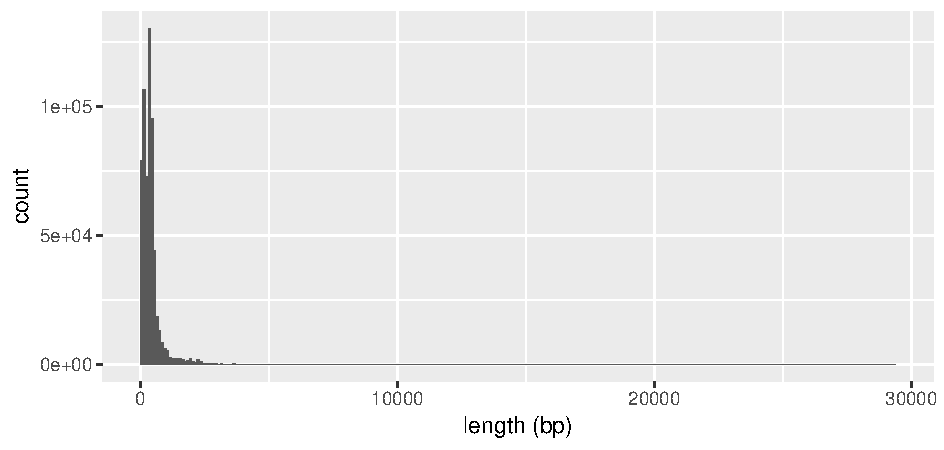
\includegraphics[scale = 1, keepaspectratio = true]{../figures/hervS2_length_hist}  
	\caption{Length distribution of elements in HERV S2}
    \label{fig:hervS2.length.hist}
\end{figure}


\section{KORA}
\label{Data:KORA}
The functional data for our analysis of gene regulatory mechanisms are made up expression, methylation and genotype data. These were collected in the light of the platform for Cooperative Health Research in the Region of Augsburg, short KORA. It contains health surveys as well as examinations of individuals of German nationality living in the area of Augsburg, Bavaria.
The objective of KORA is to track changes in health conditions over a long period in order to identify and examine the causes, effects and development of chronical diseases.

The data used in this work originates from the KORA F4 Survey, which was conducted from 2006 to 2008 and comprised samples of 3080 individuals. Of these data was available for 3020 individuals. F4 is a follow up study to the KORA S4 Survey performed from 1999 to 2001. It contains 4261 individuals. 

All measurements were performed on whole blood samples. Houseman blood counts\cite{10.3389/fgene.2016.00023} describing the composition of different cell types for each individual had previously been calculated from the methylation data. They were used to weight certain cell type specific data. 

Not all essays are available for all samples. Therefore different analyses were performed on varying sets of individuals according to availability of the required data types. A diagram of the samples available for each essay can be seen in figure \ref{fig:samples.venn}. The joint analysis, using Gaussian Graphical Models, was performed on 687 individuals that had all three essays available. 
\begin{figure}[tb]
\begin{center}
	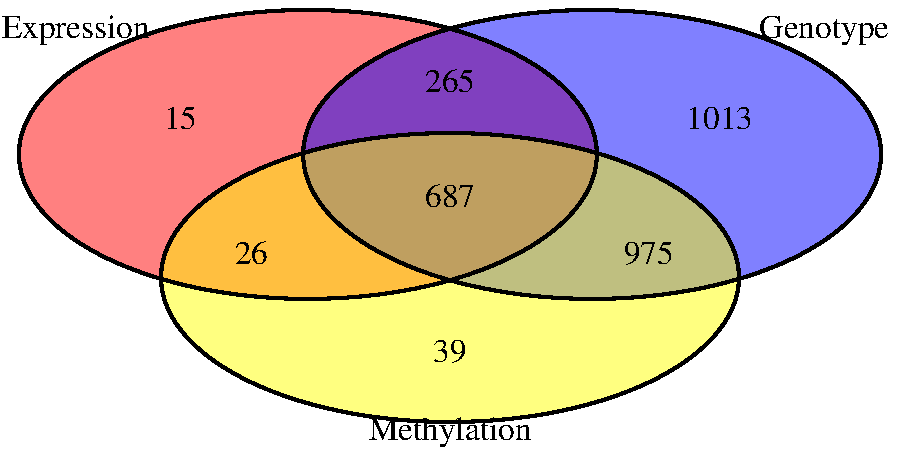
\includegraphics[scale = 1, keepaspectratio = true]{../figures/samples_venn}  
	\caption{Number of samples with genotype, expression and methylation measurements in KORA F4 Survey}
    \label{fig:samples.venn}
\end{center}
\end{figure}

\subsection{Expression}
\label{Data:Expression}
The expression data was generated using the HumanHT-12 v3.0 Gene Expression BeadChip. The chip can measure expression values for 49576 probes. However, only 47864 probes represent an actual genomic location. The remaining probes are control probes used to assess the quality of the measurements and infer the background for measurements. 

Measurements for 993 individuals are available from the KORA F4 Survey. The< comprise values for a total of 48803 probes per sample. Probes that do not map to a genomic location were excluded in all analyses, leaving 47864 probes. Of these 29521 are annotated to a total of 19288 genes. 

The available data had already been quantile normalized, corrected for the background and log-transformed. 

%TODO generate example botplots for max/min cov probes, what up with long tail?
Figure \ref{fig:expr.raw.hist.cov} shows the distribution and coefficient of variation over all probes and samples. Apart from a tail of some probes with very high expression values figure \ref{fig:expr.raw.hist.cov}A roughly resembles a standard distribution. 

\begin{figure}[tb]
	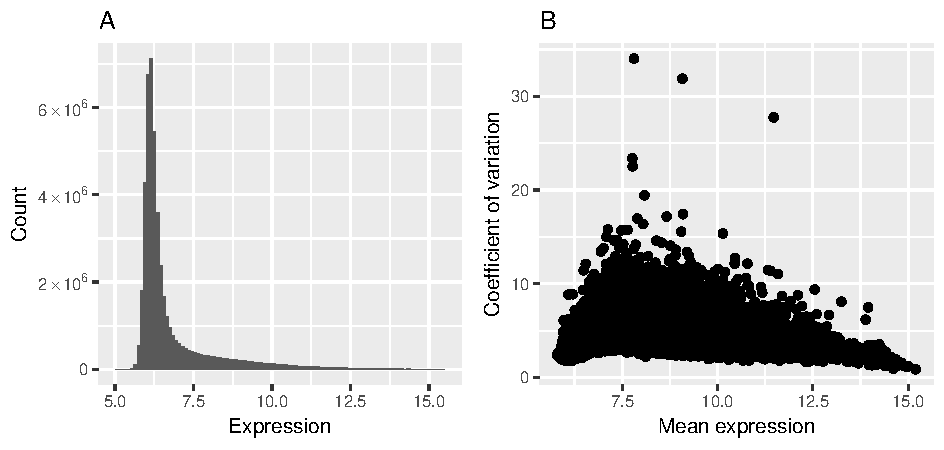
\includegraphics[scale = 1, keepaspectratio = true]{../figures/expr_raw_hist_cov}  
	\caption{Distribution of expression values (A) and coefficient of expression variation (B) of 47864 probes in 993 individuals.}
    \label{fig:expr.raw.hist.cov}
\end{figure}


Probes that could not be mapped to genes were not discarded to avoid losing data for HERV regions, which are only sparsely annotated with genes and were the focus of this work. Therefore, most analyses were performed on probe level or a mix of probes and genes. Whenever there were multiple probes mapping to the same gene, the mean of the expression values of these probes was taken as estimation of expression level for the gene. 


\subsection{Methylation}
\label{Data:Methylation}
DNA methylation was measured using the Infinium HumanMethylation450K BeadChip, which interrogates methylation levels at 485577 genomic locations. Methylation intensities had already been corrected and transformed to beta values. Beta values have a range from 0 to 1 and represent the fraction of copies of a CpG site that are methylated in a sample.

No imputation of missing measurements was performed for the methylation data. Therefore, only 44335 probes have no missing values at all and measurements in all samples available. Overall there are about 11.2 million missing values, which makes up 1.3\% of all measurements and on average 23 samples missing per probe. The histogram of proportion of missing values per probe (A) and sample (B) can be seen in figure \ref{fig:meth.na.hist}.

\begin{figure}[tb]
	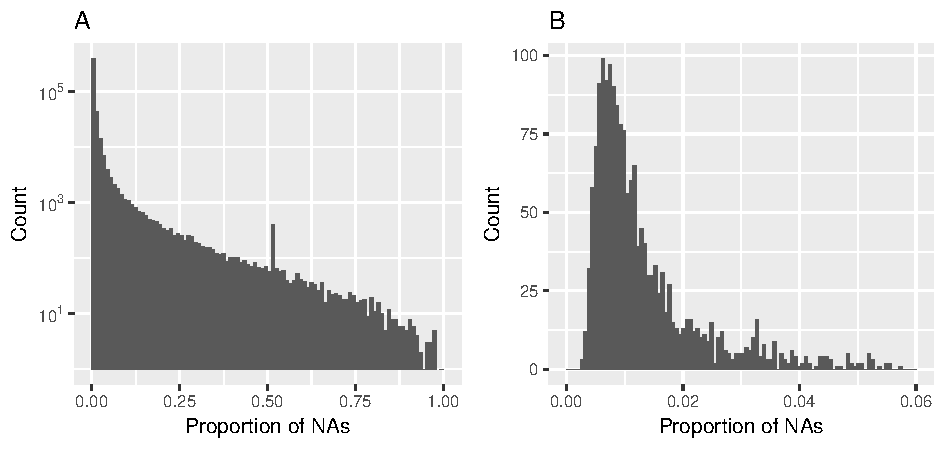
\includegraphics[scale = 1, keepaspectratio = true]{../figures/meth_na_hist}  
	\caption{Histograms of proportions of missing values per CpG-site (A) and sample (B).}
    \label{fig:meth.na.hist}
\end{figure}

%TODO find source for methylation pattern stability
Methylation data was available for 1727 individuals and 485512 sites, which make up all 'cg' and 'ch' probe type probes. The distribution of beta values and the variances over all samples and probes is shown in figure \ref{fig:meth.raw.hist.var}. As seen in figure \ref{fig:meth.raw.hist.var}A, the interrogated CpG sites tend to be either entirely methylated or unmethylated within single samples. This means that all cells in a sample have the same, stable methylation pattern, which is expected as methylation is known to be stable within a certain condition\cite{}. However, as subfigure B shows there is some variance between individuals in most CpG-sites. The low variance for very low and very high betas is explained by the fact that for a CpG site to have a mean close to 0 all samples have to have a value close to 0. Therefore, the variance also is very low.

 
\begin{figure}[tb]
	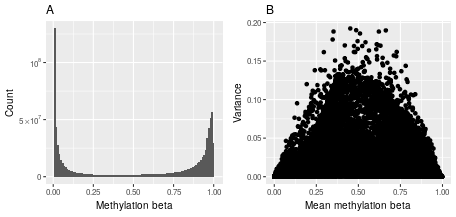
\includegraphics[scale = 1, keepaspectratio = true]{../figures/meth_raw_hist_var}  
	\caption{Distribution of all methylation beta values (A) and variance (B) of 485577 CpGs between 1727 individuals.}
    \label{fig:meth.raw.hist.var}
\end{figure}

 
\subsection{Genotypes}
\label{Data:Genotypes}
Genotyping was performed with the Affymetrix Axiom 6.0 array. On the data set used in this work genotypes had already been called using the Iluminus calling algorithm and missing values had been imputed using the IMPUTE2 software\cite{10.1371/journal.pgen.1000529}. Furthermore, imputation results had already been filtered at IMPUTE value of 0.4.  

%TODO rewrite
Additionally SNPs with a minor allele frequency of less than one percent had been removed, which allows used association analyses to be have more powerful test statistics.

In total measurements of 9533127 SNPs for 2940 individuals were available in the form of continuous dosages from 0 to 2 with 0 representing no occurrence of the SNP and 2 meaning the SNP is present in both chromosomes. Non integer values mean that different genotypes were measured in different cells in the sample and the resulting value describes the fraction of the occurrence of the variant. 

\subsection{Covariates}
\label{Data:Covariates}
Several covariates were known for each sample. They were used to correct expression and methylation values for shared effects. 

%TODO which sex is which?
The sex of all participants was known. Of the 3020 participants with any available data 1458 were SEX1 and the remaining 1562 were SEX2. The 697 individuals that had all three essays available contained 348 men/women and 339 women/men.
Further covariates specific to participating individuals are sex, age, body mass index (BMI) and white blood cell count. An overview of these covariate values for all 3020 individuals and the individuals with all three essays available is shown in table \ref{tab:covariate.overview}.


%TODO fix tables, add caption, maybe add RIN to table
\begin{table}[h!]
  	\begin{minipage}{.45\textwidth}
    \pgfplotstabletypeset[
    col sep=tab, 
    header=true,    
	columns={Covariate, Minimum, Maximum, Mean},
	columns/Covariate/.style={column type=l,string type},
	every head row/.style={before row=\hline, after row=\hline},
	every last row/.style={after row=\hline}]{../tables/full.covariate.overview.tsv}
    \end{minipage}
    \hfill
     \begin{minipage}{.45\linewidth}
    \pgfplotstabletypeset[
    col sep=tab, 
    header=true,    
	columns={Covariate, Minimum, Maximum, Mean},
	columns/Covariate/.style={column type=l,string type},
	every head row/.style={before row=\hline, after row=\hline},
	every last row/.style={after row=\hline}]{../tables/select.covariate.overview.tsv}
    \end{minipage}%
    \caption{Covariate overview}
	\label{tab:covariate.overview}
\end{table}

Finally, three experimental factors for the expression measurements, storage time, RNA integrity number (RIN), a measure that describes the degree of degradation of RNA molecules\cite{Schroeder2006}, and plate, were known.

\subsection{Methylation quantitative trait loci}
\label{Data:meQTL}
%TODO find source paper
Genotypic variants are known to effect methylation patterns in humans \cite{}. Therefore, we used previously processed methylation quantitative trait loci (meQTL) data to explore the mechanism of trans acting SNP-CpG associations. Associated pairs were used as a seed for trans-acting interaction networks.

For meQTLs a stringent definition of trans effects was used: A SNP-CpG pair was called a trans-meQTL only if they are located on different chromosomes. This definition differs from the one used for eQTM and eQTL calculation as described later. 

%TODO generate some kind of figure for meQTL numbers
The data set contained a total of 11165559 significantly associated SNP-CpG pairs. 
70709 distinct CpG-sites and 2709428 SNPs were part of at least one meQTL. On average each SNP was associated with 4.12 CpGs and each CpG was part of on average 157.91 meQTLs.

Of these 467915 pairs consisting of 3592 CpG-sites and 200761 SNPs were between different chromosomes. 


\section{Transcription factor binding}
\label{Data:tfbs}
DNA methylation plays a major role in the specifics of transcription factor binding sites\cite{Yineaaj2239}. We used transcription factor binding sites obtained from two publicly available sources to enrich information about CpG-sites of interest with transcription factors that bind nearby: 

The first source was the third version of the track "Transcription Factor ChIP-seq (161 factors) from ENCODE with Factorbook Motifs"\cite{10.1101/gr.139105.112} downloaded from the UCSC genome browser download section (\url{http://hgdownload.cse.ucsc.edu/goldenPath/hg19/encodeDCC/wgEncodeRegTfbsClustered/wgEncodeRegTfbsClusteredWithCellsV3.bed.gz}).

It combines 690 high quality ENCODE ChIP-seq data sets, which were processed with the Factorbook motif discovery and annotation pipeline\cite{10.1101/gr.139105.112}. The pipeline uses the tools MEME-ChIP\cite{10.1093/bioinformatics/btr189} and FIMO\cite{10.1093/bioinformatics/btr064} from the MEME software suite and merges discovered motifs with known motifs from Jaspar\cite{10.1093/nar/gkx1126} and TransFac\cite{10.1093/nar/gkj143} using machine learning methods and manual curation. 

The track contains a total of 438044 distinct peaks for 161 transcription factors in 91 cell types. For our analyses we filtered and combined the peaks for 23 blood related cell types. This leaves a total of 2475316 peaks for 125 transcription factors.  

The second source was the ReMap project\cite{10.1093/nar/gku1280}. It combines 395 publicly available ChIP-seq data sets covering 132 different transcription factors across 83 cell lines. ReMap uses Bowtie2\cite{10.1038/nmeth.1923} to map reads to the human genome and the tool MACS\cite{10.1186/gb-2008-9-9-r137} for peak calling. The final data set was downloaded from the ReMap website\url{(http://tagc.univ-mrs.fr/remap/download/All/filPeaks_public.bed.gz)}.

There were a total of 8905156 peaks for 131 transcription factors in the data set. After filtering for 19 blood related cell types 1372245 peaks for 35 different transcription factors remained.  

Combining both filtered data sets lead to a total of 3847561 peaks of 145 different transcription factors.

\section{Protein interaction network}
\label{Data:Protein interaction network}
Protein interaction data were used to include potential interaction partners in the generation of interaction networks.

Human protein interaction data were downloaded from the STRING database version 9\cite{Franceschini2013}. STRING is a database for direct and functional protein associations that is compiled by combining multiple sources: Experimental evidence of interaction, known pathways and protein complexes from curated databases, co-expression analysis, knowledge transfer from other species based on gene orthology, and automated text-mining of scientific literature\cite{Szklarczyk2017}. 

The data set contained 3019612 pairwise protein interactions between 16590 different proteins. For each pair associations scores for the described categories were available. Protein interactions were filtered for the availability of experimental and/or database evidence by excluding pairs with and association score of 0 in both categories, which left 375702 interactions between 12769 different proteins. 

Further filtering was performed, by excluding proteins, whose genes were not found expressed in whole blood. Therefore, expression values from RNA-seq experiments for 55 tissues in human were downloaded from the  Genotype-Tissue Expression (GTEx) Project\cite{GTExConsortium2013}. Transcripts with an RPKM (Reads per kilobase per million mapped reads) of more than 0.1 in blood were considered expressed. Interactions where one or both members were not represented by these 17343 transcripts were removed.

Finally, connected components were calculated on the network represented by the remaining pairwise interactions and all genes not within the biggest connected component were removed. The final network contained 8546 proteins and 97447 interactions. 

\section{Chromatin states}
\label{Data:Chromatin states}
%TODO rewrite somewhat - but not used right now
Chromatin state annotations were downloaded from Roadmap Epgenomics Core 15-state model (\url{http://egg2.wustl.edu/roadmap/data/byFileType/chromhmmSegmentations/ChmmModels/coreMarks/jointModel/final}). The Model provides a whole genome chromatin state annotation of 200 bp wide windows to the following 15 states: Active Transcription Start Site (TSS), Flanking Active TSS, Transcription at gene 5' and 4', Strong transcription, Weak transcription, Genic enhancers, Enhancers, ZNF genes \& repeats, Heterochromatin, Bivalent/Poised TSS, Flanking Bivalent TSS/Enhancer, Bivalent Enhancer, Repressed PolyComb, Weak Repressed PolyComb and Quiescent/Low. The model is available for 127 diverse cell lines. 

It was generated using ChromHMM v1.10\cite{10.1038/nmeth.1906} on the chromatin marks H3K4me1, H3K4me3, H3K27me3, H3K9me3, and H3K36me3. ChromHMM is based on a multivarate Hidden Markov Model. 

In this work the annotations for 27 blood related cell lines were used. When combining the annotation for a genomic location of interest like a HERV element or a SNP, houseman blood counts were used to account of the cell composition of the whole blood samples. 


\newpage
\chapter{Methods}
\label{Methods}
Most computations were done using the statistical computing environment and programing language R, version 3.4.1\cite{Rlanguage}. Pre filtering steps on large files, that could not be loaded into random access memory, were performed using the bash command "awk", which runs scripts written in the "AWK" programming language.

\section{Overlaps}
\label{Methods:Overlaps}
The main objective of this thesis was to analyze the effects of HERV elements on the regulation of cell activity. 

To identify functional features like expression probes, genes, SNPs and CpG-sites that were associated with HERV elements, overlaps between these features and elements were calculated. Features were considered to be of interest for the analysis of an HERV element, if they overlapped by at least one base pair.

The calculation was performed using the function "findOverlaps" from the Bioconductor package "GenomicRanges"\cite{10.1371/journal.pcbi.1003118}. The function allows to identify overlaps between "GRanges" objects. These were constructed from BED files for all HERV sets as well as SNPs and retrieved from the Bioconductor packages available for analyses on the expression and methylation essays, "illuminaHumanv3.db"\cite{illuminaHumanv3.db} and "FDb.InfiniumMethylation.hg19"\cite{FDb.InfiniumMethylation.hg19} respectively.

The search for overlapping features was also performed on "GRanges" objects including all HERV elements as well as the 1kb or 2kb flanking regions of all elements. This was done to include functional features, that while not directly within HERV regions, are still likely to be influenced by them. Furthermore, this analysis was performed on all three HERV sets.

\section{Data normalization}
\label{Methods:Data normalization}
Before expression and methylation values were used for analyses, they were corrected for batch effects. For this we used the available covariates to calculate linear models and regress out the respective residuals. The model used for expression values is shown in equation \ref{eq:expr.res.model} and considers the covariates age, sex, RNA integrity number (RIN), plate and storage time. The model for methylation values, shown in equation \ref{eq:meth.res.model},
includes the cell composition for the five blood cell types known from the houseman blood counts, as well as the first 20 principal components of the Illumina 450k array control-probes. 
\begin{equation}
\label{eq:expr.res.model}
Expr \sim 1+age+sex+RIN+plate+storage.time
\end{equation}
\begin{equation}
\label{eq:meth.res.model}
Meth \sim 1+CD4T+CD8T+NK+Bcell+Mono+PC_1+...+PC_{20}
\end{equation}


\section{eQTL/eQTM calculation}
\label{Methods:eQTL/eQTM calculation}
As a preliminary analysis to interrogate the effect of genotype and methylation variants on expression, expression quantitative trait loci (eQTL) and expression quantitative trait methylation (eQTM) were calculated.

In the following paragraphs the calculation of eQTLs will be described. The calculation of eQTMs was performed analogously, the only difference being that methylation residuals were supplied instead of SNP dosages.

Calculations were performed using the Bioconductor package MatrixEQTL\cite{10.1093/bioinformatics/bts163}. MatrixEQTL tests for association of SNP-transcript pairs.  

We set the parameter \texttt{useModel = modelLINEAR}, which leads to the use of an  additive linear model. The association is modeled as simple linear regression and the absolute value of the sample correlation is used as test statistic.

After calculating the test statistics the p-values for all pairs that pass a defined significance threshold are calculated. These are corrected multiple testing using a Benjamini-Hochberg procedure\cite{10.2307/2346101}, adapted for not recording all p-values, as shown in equation \ref{eq:matrix.eqtl.transformation}

MatrixEQTL is rather efficient because it manages to reduce the calculation of the sample correlation over all SNPs and transcripts to one single large matrix multiplication. This is achieved by transforming the genotype and transcription values. 

MatrixEQTL also allows to include covariates in the QTL calculation. As the expression and methylation values used are residuals and therefore already corrected this option is not used. Furthermore, MatrixEQTL can differentiate between cis- and trans-interactions based on distance. The maximal distance to consider a pair on the same chromosome as cis was set to 500 kb. 
%TODO motivate cis-distance

The p-value threshold for significant cis-QTLs during calculation was set to $10^{-6}$ and $10^{-8}$ for trans. As this cutoff is used for uncorrected p-values, a more stringent threshold is set for trans QTLs to account for the bigger number of possible pairs. 



\section{Functional Analysis of Gene Sets}
\label{Methods:Functional Analysis of Gene Sets}
In multiple analyses functional Gene Ontology enrichments were performed.

First a set of all GO annotations with any evidence code for gene symbols  was retrieved from the Bioconductor package AnnotationDbi\cite{AnnotationDbi}. 

Then a hypergeometric test\cite{GOstats} for overreprensentation was performed on a set of genes of interest. A custom background set of genes specific to the analysis was given for each enrichment. Finally, the p-values for overrepresented GO terms were adjusted for multiple testing using the Holm method\cite{10.2307/4615733}. Terms with an adjusted p-value of less than 0.05 were considered significantly overrepresented. 

\section{Gaussian Graphical Models}
\label{Methods:Gaussian Graphical Models}
In this work Gaussian Graphical Models (GGMs) on multiomics data with a connection to HERV elements were used to investigate the effects and effect pathways of changes in HERV elements. The calculation of GGMs was performed using the R package "BDgraph" version 2.44\cite{Mohammadi2015BDgraphAR}. First I will shortly go over the theoretical background and the method, following Mohammadi and Wit\cite{Mohammadi2015,Mohammadi2015BDgraphAR}. Then I will elaborate on how I defined the data sets to generate GGMs on.

\subsection{Methodological Background}
In Gaussian Graphical Models, random variables are represented by nodes. Conditional dependence relationships, or partial correlations,  between these variables are represented as undirected edges in a graph $G=(V,E)$, where $V=\{1,2, ..., p\}$ is a set of nodes and $E \subset V \times V$ the set of edges. A zero mean Gaussian Graphical model with respect to graph G is defined as

\begin{equation}
\mathcal{M}_G = \lbrace \mathcal{N}_p(0,\Sigma|K  \Sigma^{-1} \in \mathbb{P}_G \rbrace
\end{equation}

where $\Sigma$ is the covariance matrix, its inverse $K$ is the precision matrix and $\mathbb{P}_G$ is the cone of symmetric positive definite matrices with elements $K_{ij}$ equal to zero for all $(i,j)\notin E$. This means the random variables representing our data are assumed to follow the multivariate Gaussian distribution $\mathcal{N}(\mu, K^{-1})$, where the mean $\mu$ is zero.

With $Z = (Z^{(1)}, ..., Z^{(n)})$ being the observed data of $p$ independent samples, the likelihood function is
\begin{equation}
Pr(Z|K,G) \propto |K|^{n/2} exp\left\lbrace-\frac{1}{2}tr(KU)\right\rbrace,
\end{equation}
where $U = Z^TZ$.

As for multivariate Gaussian distributions conditional dependence is a direct representation of partial correlation\cite{10.1111/j.1467-842X.2004.00360.x}, we will only use the former going forward.

Conditional independence in the model is represented by the precision matrix in the form that two variables $i$ and $j$ are conditionally independent given the remaining variables, if and only if $K_{ij} = 0$. Therefore, the nonzero entries of $K$ correspond to links in the graph $G$.  

As mentioned in section \ref{Introduction:Effect network analysis}, the space of possible graphs is too big to explore exhaustively. When considering a case with as low as $p = 50$ variables, there are $2^{p(p-1)/2} > 10^{300}$ possible graphs. Therefore a heuristic approach is necessary. 

In the used implementation of GGM calculation the space of possible graphs and precision matrices is explored by a birth-death Markov chain Monte Carlo (BDMCMC) method. It is based on a continuous time Markov process, where jumps to a larger or a smaller dimension occur based on birth and death rates, that are chosen so that the stationary distribution of the Markov chain represents the chosen posteriori distribution.

More specific in the case of Graphical Models a birth event represents the addition of an edge $e = (i,j) \notin E$ and leads the process to a new state $(G^{+e}, K^{+e}$, where $G^{+e} = (V, E \cup \{e\})$, and $K^{+e}$ is equal to $K$ except for the positions $\lbrace (i,j), (j,i), (j,j) \rbrace$.

Analogously a death event represents the deletion of an edge $e = (i,j) \in E$ and leads the process to a new state $(G^{-e}, K^{-e}$, where $G^{-e} = (V, E \setminus \{e\})$, and $K^{-e}$ is equal to $K$ except for the positions $\lbrace (i,j), (j,i), (j,j) \rbrace$.

These events are considered to be independent Poisson processes. Birth and death rates are conditional to the joint posterior distribution of a graph G and precision matrix K, $Pr(K,G|Z)$.

The birth-rates and death-rates are defined as

\begin{equation}
\beta _e(K)=min\left\lbrace \frac{Pr(G^{+e}, K^{+e}|Z)}{Pr(G,K|Z)},1 \right\rbrace \text{, for each }  e \notin E,
\end{equation}

\begin{equation}
\delta _e(K)=min\left\lbrace \frac{Pr(G^{-e}, K^{-e}|Z)}{Pr(G,K|Z)},1 \right\rbrace \text{, for each }  e \in E,
\end{equation}

As birth and death rates are independent the total birth and death rates are

\begin{equation}
\beta(K) = \sum_{e \notin E}\beta_e(K),
\end{equation}
 
\begin{equation}
\delta(K) = \sum_{e \in E}\delta_e(K).
\end{equation}

The time between successive events is exponentially distributed and has the mean $1/(\beta(K)+\delta(K))$. Therefore, the probability of a birth or death event is given by

\begin{equation}
Pr(\text{birth of link e}) = \frac{\beta_e(K)}{\beta(K) + \delta(K)} \text{, for each } e \notin E,
\label{eq:birth.prob}
\end{equation}

\begin{equation}
Pr(\text{death of link e}) = \frac{\delta_e(K)}{\beta(K) + \delta(K)} \text{, for each } e \in E.
\label{eq:death.prob}
\end{equation}

The joint posterior distribution of a graph $G$ with the precision matrix $K$ is 

\begin{equation}
Pr(K,G|Z) \propto Pr(Z|K) Pr(K|G) Pr(G)
\end{equation}

$Pr(Z|K)$ is the likelihood and already defined. The default for the prior of the graph is $Pr(G)=\frac{1}{|\mathcal{G}|}$, where $\mathcal{G}$ is the graph space. Alternatively $Pr(G)$ can be supplanted by a distribution representing prior information of relationships between variables, if available. Finally, the prior distribution for the precision matrix is defined to be the G-Wishart distribution $W_G(b,D)$ with the following density:

\begin{equation}
Pr(K|G) = \frac{1}{I_G(b,D)}|K|^{\frac{b-2}{2}}exp\left\lbrace-\frac{1}{2}tr(DK)\right\rbrace 1(K \in \mathbb{P}_G),
\end{equation}

where $b>2$ is the degrees of freedom, $D$ is a symmetric positive definitive matrix, $I_G(b,D)$ is the normalizing constant with respect to the graph $G$ and $1(x)$ is 1 if $x$ is true, and 0 otherwise.

\newpage
The used implementation of GGMs considers the G-Wishart distribution $W_G(b,D)$ to be a prior distribution for the precision matrix $K$ with the following density:

\begin{equation}
Pr(K|G) = \frac{1}{I_G(b,D)}|K|^{\frac{b-2}{2}}exp\left\lbrace-\frac{1}{2}tr(DK)\right\rbrace 1(K \in \mathbb{P}_G),
\end{equation}

where $b>2$ is the degrees of freedom, $D$ is a symmetric positive definitive matrix, $I_G(b,D)$ is the normalizing constant with respect to the graph $G$ and $1(x)$ is 1 if $x$ is true, and 0 otherwise.

In the calculation of GGMs with the package BDgraph the following steps are repeated for a given number of iterations:

First The birth and death rates as well as the waiting time is calculated. Then a jump is simulated according to the probabilities in equations \ref{eq:birth.prob} and \ref{eq:death.prob} and an edge is added or removed. Finally, the precision matrix for the new graph is sampled. This is done using a sampler defined in \cite{Mohammadi2015}, that I will not elaborate on.  

The output of the calculation consists of the graphs, precision matrices and waiting times for each iteration. The posterior probabilities of all visited graphs are estimated by the total waiting time on each graph during the iterations as shown in figure \ref{fig:bdgraph.waiting.graph}. This means a graph is considered more likely when it was visited multiple times and/or the total birth and death rates when at this graph were low leading to long waiting times. The approach usually takes some time to converge close to the posterior distribution. Therefore, BDgraph offers the the function to define a number of iterations, that are used as "burn-in" period, which are not considered for the calculation of graph probabilities.  

\begin{figure}[b!]
\begin{center}
	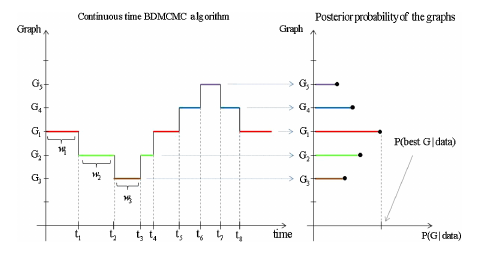
\includegraphics[scale=1.2, keepaspectratio = true]{../figures/bdgraph_waiting_graph}
	\end{center}
	\caption{}
	\label{fig:bdgraph.waiting.graph}
\end{figure}

An extension to GGMs that allows the method to be used on both discrete and continuous variables is called Gaussian copula graphical modeling. This is done by introducing a multivariate Gaussian latent variable that transform the raw data in way that makes it usable in the calculation of GGMs. 

%The G-Wishart prior also is a conjugate prior the to likelihood function of the multivariate Gaussian distribution. Therefore, the posterior distribution of $K$ is 
%\begin{equation}
%Pr(K|Z,G) = \frac{1}{I_G(b^*,D^*)}|K|^{\frac{b^*-2}{2}}exp\left\lbrace-\frac{1}{2}tr(D^*K)\right\rbrace ,
%\end{equation}
%where $b^* = b+n$ and $D^* = D+S$. This is once again a G-Wishart distribution, $W_G(b^*,D^*)$.
\subsection{Data collection}
\label{Methods:Data collection}
Gaussian Graphical models have the severe limitation, that sample covariance and correlation matrices are well conditioned only when the number of variables is smaller than the number of samples\cite{Schaefer2005}. Therefore, it is absolutely necessary to perform a pre-selection of included entities when calculating GGMs on our multiomics data set.

We performed two mechanisms of selecting node sets. Both are anchored in trans-acting SNP-CpG interactions as well as a relationship to HERV elements. 

The first way starts of with a SNP that lies within a HERV element and has significant associations with at least 5 CpG sites located on another chromosome. These CpGs are added to the analysis.  To include genes, that are potentially associated with this SNP, all expression probes within a 250 kb flanking region up- and downstream of the sentinel SNP are included. Analogously to find genes that are likely to be affected by methylation changes, for each associated CpG all overlapping probes and the first up- and downstream probe each within a distance of less than 250 kb are added. To include transcription factors, whose binding might be affected by DNA methylation changes, all TFs that have a binding site within 100 bp of a CpG of interest are added. Finally, in an attempt to connect genes around the sentinel SNP with genes around the methylation sites or transcription factors, we used the String network described in section \ref{Data:String protein interactions}. We calculated the shortest path from a representative SNP gene to any TF or CpG gene and included all genes on this path.

%TODO write caption
\begin{figure}[b!]
	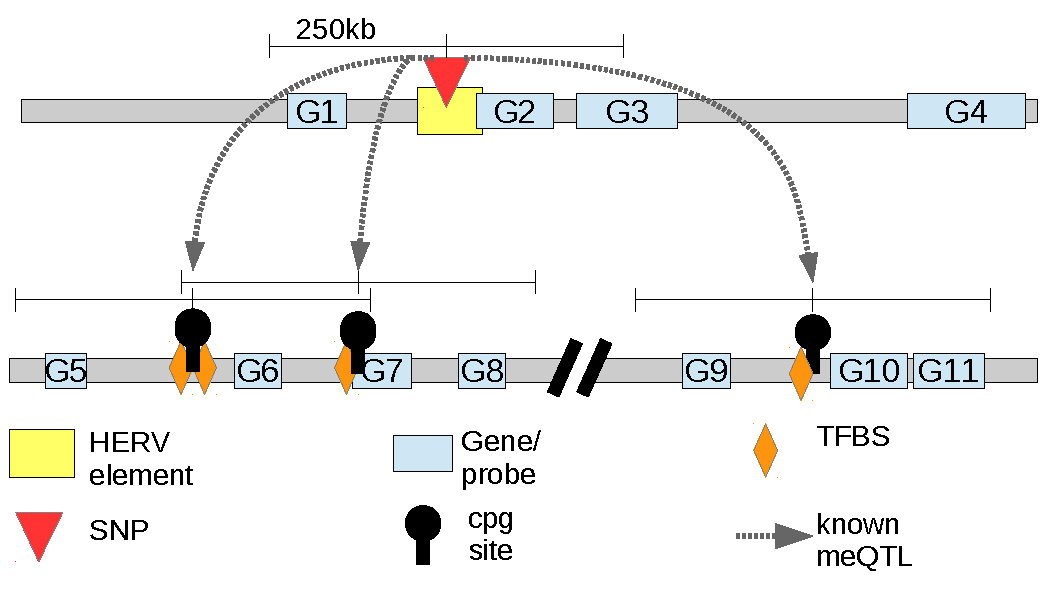
\includegraphics[scale=0.86, keepaspectratio = true]{../figures/ggm_data_collect_snp_scheme}
	\caption{}
	\label{fig:ggm.data.collect.snp.scheme}
\end{figure}

The schematic representation of the selection starting from an example SNP is shown in figure \ref{fig:ggm.data.collect.snp.scheme}

The second approach of data collection, shown in figure \ref{fig:ggm.data.collect.cpg.scheme}, starts with an CpG-site within a HERV element, that is part of a trans-meQTL. First, if any other measured CpGs lie within the same HERV and are part of a trans-meQTL, they are added to the analysis. Then for each CpG of interest the most strongly associated SNP that lies on another chromosome is added. Other CpGs that are in a trans-meQTL with these SNps are included as well. Finally neighboring genes, transcription factors and shortest path genes are included according to the same criteria as in the first approach.

%TODO write caption
\begin{figure}[b!]
	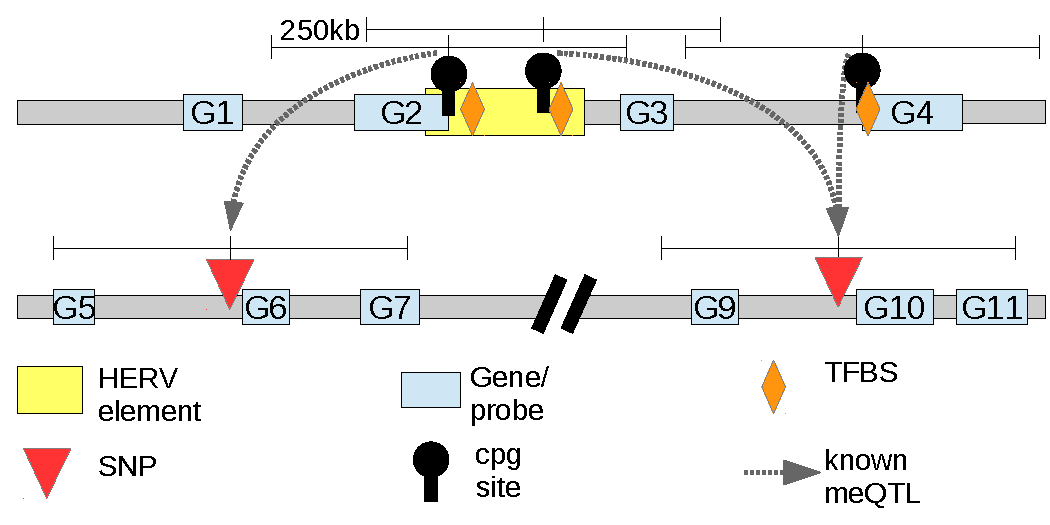
\includegraphics[scale=0.86, keepaspectratio = true]{../figures/ggm_data_collect_cpg_scheme}
	\caption{}
	\label{fig:ggm.data.collect.cpg.scheme}
\end{figure}

For both approaches data sets that contained too few members were excluded as follow. Sets with less than one gene or probe neighboring a SNP and one neighboring a CpG-site were removed. Furthermore, if no transcription factor and no shortest path gene was found, the set was excluded. Therefore, each GGM calculated contained at least 5 entities.

\subsection{GGM calculation and filtering}
\label{Methods:GGM calculation and filtering}
The BDgraph main method "bdgraph" was used to calculated the GGMs on the data sets that were just defined. I used the parameters, \texttt{'method = "gcgm"}, which leads to the use of the extension for mixed data. As algorithm I used the package default 'algorithm = "bdmcmc". The number of iterations was set to \texttt{'iter = 50000'}, while the burn-in period was \texttt{'burnin = 25000'}. "bdgraph" was run with a prior edge distribution of 'g.prior = 0.5'. The starting graph was set to \texttt{'g.start = "empty"'}, which means the calculation is started in an unconnected graph. Finally, the degrees of freedom for the G-Wishart distribution used to calculate the prior of the precision matrix was chosen as \texttt{'prior.df = 3'}.

Due to large number and size of calculated GGMs no manual analyses of all networks was possible. Therefore, multiple criteria were defined to identify potentially interesting GGMs.

First the edges in the network were filtered for an edge inclusion probability of more than 0.9. Then the connected components were determined. Networks, whose seed SNP or at least one seed CpG were not part of the biggest connected component, were excluded from the analysis. 

Then the numbers of CpGs/SNPs, CpG/SNP genes and probes, transcription factors and path genes included in the biggest connected component were counted. As for the data prior to GGM calculation, networks with less than one SNP/CpG gene or probe and no shortest path gene or transcription factor were removed. 

Furthermore, the the amount of CpG and SNP genes, that had an edge to the CpG/SNP that caused them to be included in the analysis was determined. Finally, the eQTL and eQTM results described in sections \ref{Results:eQTLs} and \ref{Results:eQTMs} were used to assess how many of the identified associations were found in the network, either as being part of the same connected component or a direct edge. 

%TODO include expected/hoped for GGM structure, elaborate on why certain edges are interesting

A manual inspection of these criteria was performed in order to select which GGMs would be the target of detailed manual analysis. 

\newpage
\chapter{Results}
\label{Results}
\section{Normalized Data}
\label{Results:Normalized Data}
%TODO expand and source why normal dist
The distributions of the expression and methylation residuals, calculated as described in chapter \ref{Methods:Data normalization}, over all probes and samples can be seen in figure \ref{fig:expr.meth.res.hist}. As expected the residuals follow a normal distribution. This is important for the calculation of the Gaussian graphical models, as the normal distribution of the data is one of base assumptions for Gaussian graphical models\cite{Mohammadi2015}.

\begin{figure}[b!]
	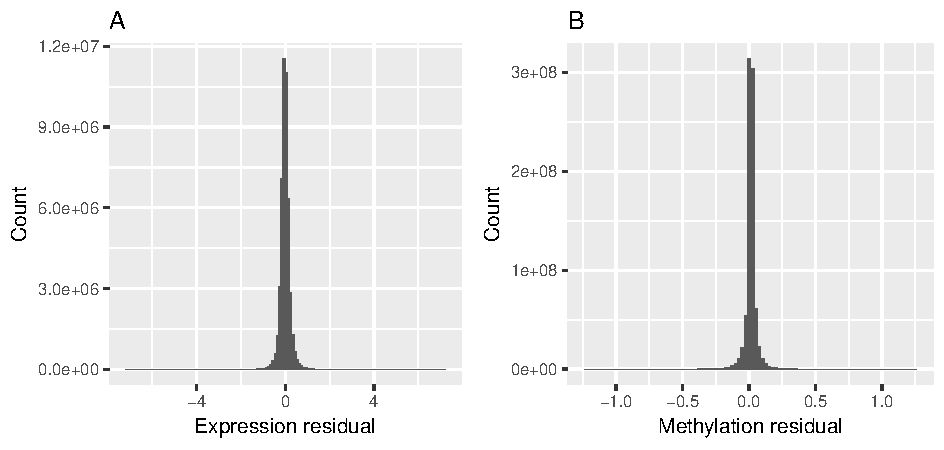
\includegraphics[scale=1, keepaspectratio = true]{../figures/expr_meth_res_hist}
	\caption{Distribution of expression (A) and methylation (B) residuals over all samples and probes}
	\label{fig:expr.meth.res.hist}
\end{figure}

\section{HERV region features}
\label{Results:HERV region features}
In this section I will describe the expression probes that overlap with and the cpgs and SNPs that lie within any HERV element and/or their flanking regions. The results for the set of all endogenous retroviral elements, HERV set 2, without flanking regions are described in detail. The results for the other sets defined in chapter \ref{Data:HERV annotation} and including flanking regions will be shown in tables or in the supplementary data.

\subsection{Expression}
\label{Results:Expression}

\begin{figure}[tb]
	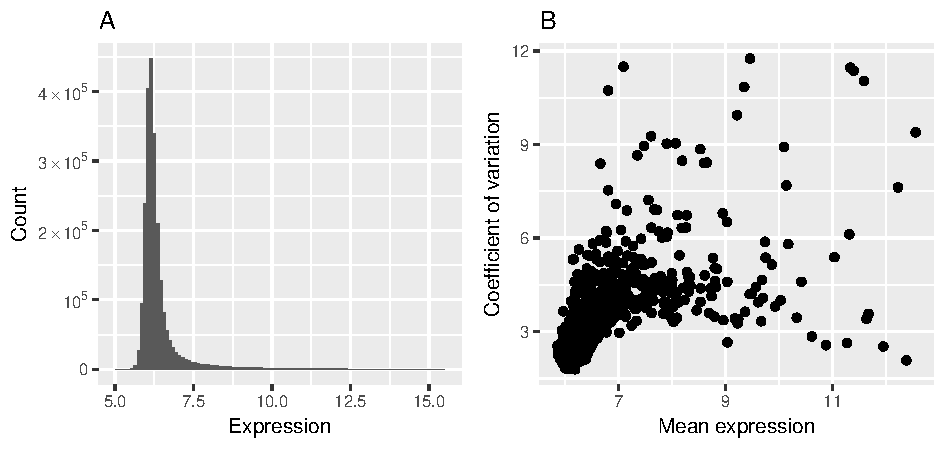
\includegraphics[scale = 1, keepaspectratio = true]{../figures/hervS2_expr_raw_hist_cov}  
	\caption{Distribution of expression values (A) and coefficient of expression variation (B) of 2343 expression probes overlapping with HERV S2 in 993 individuals.}
    \label{fig:hervS2.expr.hist.cov}
\end{figure}

A total of 2343 expression probes overlap directly with at least one of 2271 HERV elements from HERV S2. This means ca 4.50\% of all expression probes overlap with HERV elements and expression measurements are known for parts of ca 0.37\% of all HERV elements.

The distribution of expression values of the probes overlapping with HERV elements, as shown in figure \ref{fig:hervS2.expr.hist.cov}A is almost identical to the distribution of all probes (figure \ref{fig:expr.raw.hist.cov}A). The coefficient of variation (figure \ref{fig:hervS2.expr.hist.cov}B), however, is lower on average for the considered subset compared to the whole set of probes (figure \ref{fig:expr.raw.hist.cov}B).

Of these 2343 probes 510 were annotated to one of 449 different genes. I performed a GO enrichment for the biological process ontology on these genes with the set of all genes with available expression data as background. After correcting for multiple testing only the term defense response (GO:0006952, $p-value=1.37*10^{-5}$, $fdr=0.047$) was significantly enriched.

\begin{table}[h!]
  \begin{center}
  \resizebox{\textwidth}{!}{
    \pgfplotstabletypeset[
    col sep=tab, 
    header=true,    
	columns={Term ID, Term, p, fdr},
	columns/Term ID/.style={column type=l,string type},
	columns/Term/.style={column type=l,string type},
	every head row/.style={before row=\hline, after row=\hline},
	every last row/.style={after row=\hline}]
    {../tables/hervS2.2kb.expr.enrichment.tsv}}
  \end{center}        
	\caption{Significantly enriched GO biological process terms among genes overlapping with HERV S2.}
	\label{tab:hervS2.2kb.expr.enrichment}
\end{table}

However, when including the 2kb flanking regions of HERV S2 and performing the GO enrichment on the 5518 identified genes, the six GO terms shown in table \ref{tab:hervS2.2kb.expr.enrichment} are significantly overrepresented. They are all connected to defense or immune response.

The results for all HERV sets and including flanking regions is shown in table \ref{tab:expr.overlap.counts}.

\begin{table}[h!]
  \begin{center}
    \pgfplotstabletypeset[
    col sep=tab, 
    header=true,    
	columns={Set,S1,S1.1kb,S1.2kb,S2,S2.1kb,S2.2kb,S3,S3.1kb,S3.2kb},
	columns/Set/.style={column type=l,string type},
	every head row/.style={before row=\hline, after row=\hline},
	every last row/.style={after row=\hline}]
    {../tables/expr.overlap.overview.tsv}
  \end{center}        
	\caption{Overview of expression probes overlapping with different HERV sets and flanking regions. "Pairs" describes the total number of overlaps occurring, "HERVs" and "Probes" are the number of distinct HERV elements/expression probes that are part of at least one overlap.}
	\label{tab:expr.overlap.counts}
\end{table}

\subsection{Methylation}
\label{Results:Methylation}
\begin{figure}[tb]
	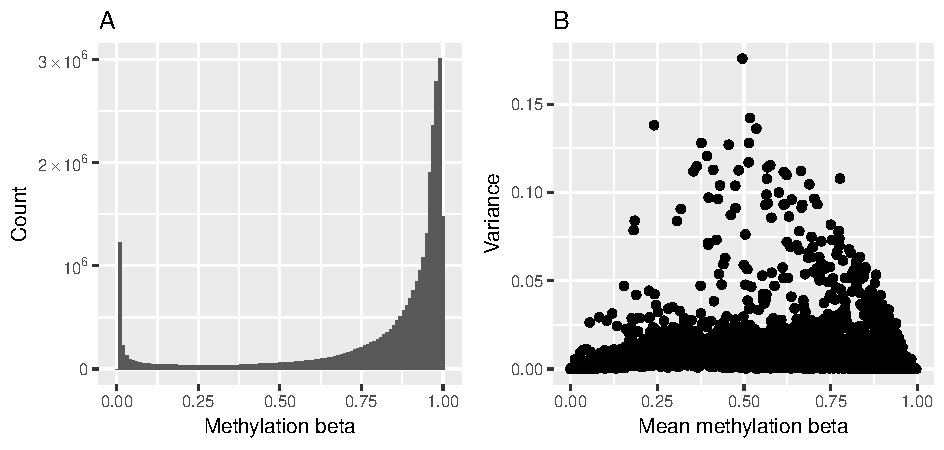
\includegraphics[scale = 1, keepaspectratio = true]{../figures/hervS2_meth_raw_hist_var}  
	\caption{Distribution of methylation beta values (A) and coefficient of methylation variation (B) of 17077 GpG-sites located within HERV S2 in 1727 individuals.}
    \label{fig:hervS2.meth.hist.var}
\end{figure}
17077 CpG sites, equaling 3.52\% of all measured CpGs, were found within HERV S2 and 12871 distinct HERV elements (2.10\%) contain at least one interrogated CpG site.

CpGs associated with HERV S2, as shown in figure \ref{fig:hervS2.meth.hist.var}A, tend to be highly methylated. The variance also is (figure \ref{fig:hervS2.meth.hist.var}B) is on average lower than the one for all CpG-sites (figure \ref{fig:meth.raw.hist.var}B).

The number of CpG sites within all HERV sets and including flanking regions is shown in table \ref{tab:meth.overlap.counts}

\begin{table}[h!]
  \begin{center}
    \resizebox{\textwidth}{!}{
    \pgfplotstabletypeset[
    col sep=tab, 
    header=true,    	columns={Set,S1,S1.1kb,S1.2kb,S2,S2.1kb,S2.2kb,S3,S3.1kb,S3.2kb},
	columns/Set/.style={column type=l,string type},
	every head row/.style={before row=\hline, after row=\hline},
	every last row/.style={after row=\hline}]
    {../tables/meth.overlap.overview.tsv}}
  \end{center}        
	\caption{Overview of CpGs overlapping with different HERV sets and flanking regions. "Pairs" describes the total number of overlaps occurring, "HERVs" and "CpGs" are the number of distinct HERV elements/GpG sites that are part of at least one overlap.}
	\label{tab:meth.overlap.counts}
\end{table} 
\subsection{Genotypes}
A total of 890780 the considered SNPs are located within elements of HERV S2. This constitutes 9.34\% of all SNPs. These SNPs are found in 330744 distinct HERV elements. Therefore, 53.99\% contain at least one SNP.

The results for all sets and flanking regions are shown in table \ref{tab:snp.overlap.counts}

\begin{table}[h!]
  \begin{center}
    \resizebox{\textwidth}{!}{
    \pgfplotstabletypeset[
    col sep=tab, 
    header=true,    
	columns={Set,S1,S1.1kb,S1.2kb,S2,S2.1kb,S2.2kb,S3,S3.1kb,S3.2kb},
	columns/Set/.style={column type=l,string type},
	every head row/.style={before row=\hline, after row=\hline},
	every last row/.style={after row=\hline}]
    {../tables/snp.overlap.overview.tsv}}
  \end{center}        
	\caption{Overview of SNPs overlapping with different HERV sets and flanking regions. "Pairs" describes the total number of overlaps occurring, "HERVs" and "SNPs" are the number of distinct HERV elements/SNPs that are part of at least one overlap.}
	\label{tab:snp.overlap.counts}
\end{table} 

The distribution of number of SNPs found in each HERV element are shown in figure \ref{fig:hervS2.snp.hist}A. A total of 2423 HERV elements had more than 20 within its boundaries and were not shown in the figure. The maximum number of SNPs found in a single HERV element was 368. This HERV element, however, is unusually long at 7003 bp. 

In figure \ref{fig:hervS2.snp.hist}B the density of SNPs per base pair of its HERV element are shown. 356 HERV elements that contained more than 0.05 SNPs per base pair were excluded from this figure.

\begin{figure}[tb]
	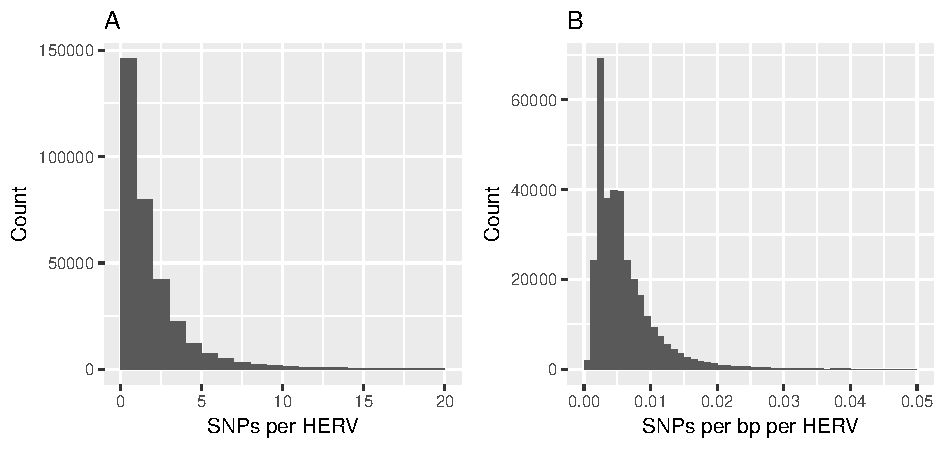
\includegraphics[scale = 1, keepaspectratio = true]{../figures/hervS2_snp_hist}  
	\caption{}
    \label{fig:hervS2.snp.hist}
\end{figure}


%\subsection{Chromatin states}
%Data in /storage/groups/groups\textunderscore epigenreg/users/julian.schmidt ...

\section{eQTLs}
\label{Results:eQTLs}
Associations were calculated for 156.4 millions cis acting SNP-expression probe pairs and 456.1 billion possible pairs in trans. 

812147 of these cis-pairs were significantly associated with p-values of $10^{-6}$ or less. These significant eQTLs have a false discovery rate of less than $1.93*10^{-4}$. A total of 551728 distinct SNPs and 4903 expression probes were part of at least one cis-eQTL. 4145 of these probes are annotated to 3552 different genes. The remaining 
758 could not be assigned to a specific gene.

There were a total of 1511235 significant trans-eQTLs with an p-value of less than $10^{-8}$ and a FDR of less than $3.02*10^{-4}$. These are made up by 229332 distinct SNPs and 21338 expression probes. 11505 of the probes found in at least one trans-eQTL are annotated to 9389 different genes, while 9767 probes are not assigned to a gene.

In a previous work Schramm et al. \cite{10.1371/journal.pone.0093844} calculated eQTLs on expression and genotype data from 2,708 subjects, including 890 KORA F4 samples. They found significant cis-eQTLs for 4116 probes and considered only the pair of the most strongly associated SNPs with the probe. Of these pairs 2680 were also found in my analysis. 

Figure \ref{fig:global.eqtl.heatmap}A shows the fraction of significant to all possible  SNP-expression probe pairs, mapped to 10 Mpb windows. As expected the values at the diagonal are comparatively higher, containing all cis-eQTLs. 

\begin{figure}[tb]
	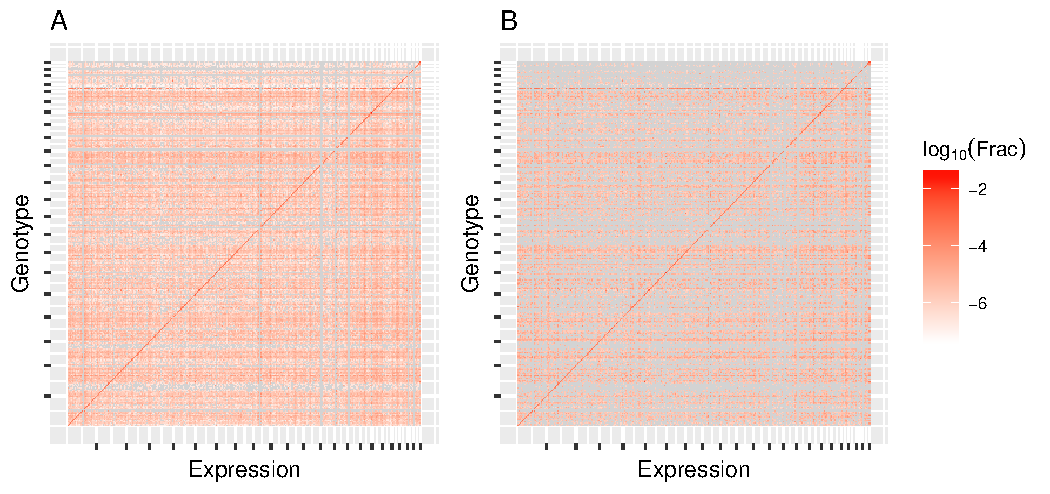
\includegraphics[scale = 1, keepaspectratio = true]{../figures/eqtl_all_herv_heatmap}  
	\caption{Fraction of SNP-expression probe pairs that were significantly associated sorted into bins according to their genomic locations. Ticks on the axis denote chromosome boundaries. Grey means there were no eQTLs in the given pair of bins. A considers all eQTLs and pairs, while B is limited on the ones whose SNP and/or expression probe are connected to HERV set 2.}
    \label{fig:global.eqtl.heatmap}
\end{figure}

The expression residual signatures of wildtype, heterogeneous and homogeneous mutated SNP site for the two eQTLs with the best and worst p-values in cis and trans are shown in figure \ref{fig:best.worst.eqtl.boxplot}. The eQTLs with the best p-values in subfigures A and C show clear distinctions between the different SNP variants. While there is a small trend between variants in subfigures B and D, the distributions of expression residuals are rather similar.    

%TODO write caption
\begin{figure}[tb]
	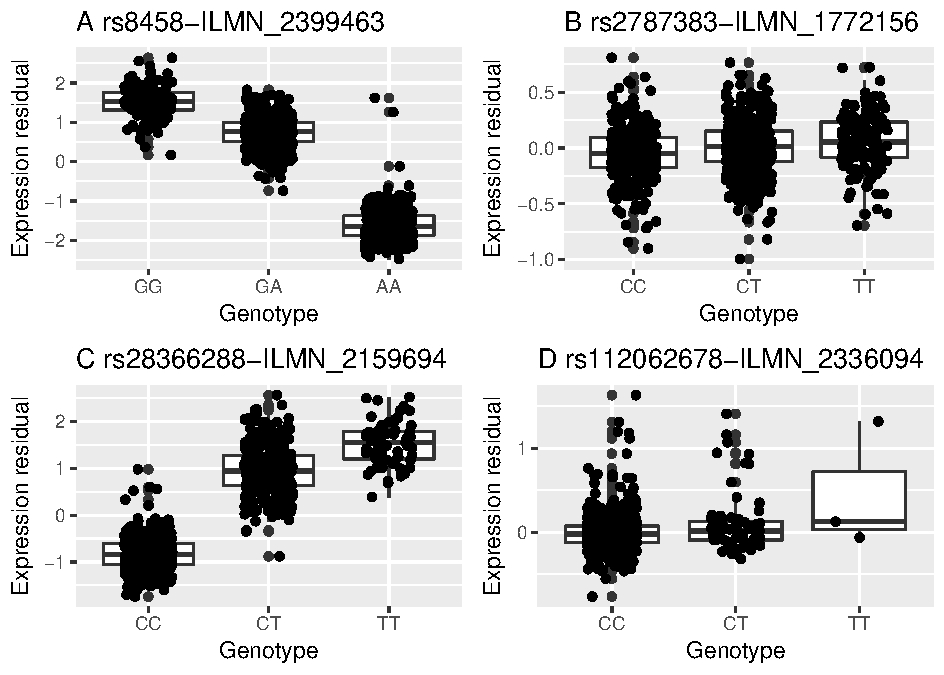
\includegraphics[scale = 1, keepaspectratio = true]{../figures/best_worst_eqtl_boxplots.pdf}  
	\caption{}
    \label{fig:best.worst.eqtl.boxplot}
\end{figure}

45862 of the SNPs and 166 of the expression probes found in at least one cis-eQTL were located within HERV S2. When considering all significant associations, where either the SNP or the expression probe lie within a HERV element, a total of 112604 pairs remained. They were made up by 3551 different expression probes, annotated to 2638 genes, and 80573 SNPs. 

There were 5855 cis-eQTLs between one of 4748 SNPs within a HERV element and one of 128 expression probes, that overlap with a HERV element. 

When limiting trans-eQTLs to the ones that contain a HERV S2 related SNP (23396) and/or expression probe (1227), 240301 remained, comprising 14573 unique expression probes (6357 genes) and 56672 SNPs. In 9177 of these pairs both members were HERV related. 

The fraction of HERV S2 related SNP-expression probe pairs that proved to be significantly associated is shown in figure \ref{fig:global.eqtl.heatmap}B. Due the smaller number of pairs, there were more cells having no data available. The general fraction of significant eQTLs was lower than when considering all eQTLs. However, the positional distribution was rather similar, with the strong diagonal containing all cis-eQTLs being clearly visible.  

A GO enrichment was performed on all 8211 genes associated to HERV related eQTLs using the set of all genes found in eQTLs as background. However, there were no significantly enriched genes. 

\section{eQTMs}
\label{Results:eQTMs}
When calculating expression quantitative trait methylation there were a total of 13.88 millions CpG-expression probe pairs within a distance of 50 Kpb or less of each other. The number of potential trans-acting pairs equaled around 23.22 billions. 

Calculating eQTMs with a significance threshold of $10^{-6}$ for cis resulted in 8187 significant associations ($fdr<1.7*10^{-4}$) consisting of 5957 distinct CpG sites and 1959 different expression probes. 1658 of these probes are annotated to 1461 genes, while there are no gene annotations for the remainder. 

361485 of the potential trans-action CpG-expression probe pairs proved to be significant at a p-value threshold of $10^{-8}$ ($fdr<6.5*10^{-4}$). These trans-eQTLs are made up by 48206 CpGs and 11673 expression probes, for which 5738 gene annotations are available. 

The fractions of potential CpG-expression probe pairs that were significantly associated between their genomic locations are shown in figure \ref{fig:global.eqtm.heatmap}A. In contrast to the eQTL results there is only a weaker preference for cis interactions. 

\begin{figure}[tb]
	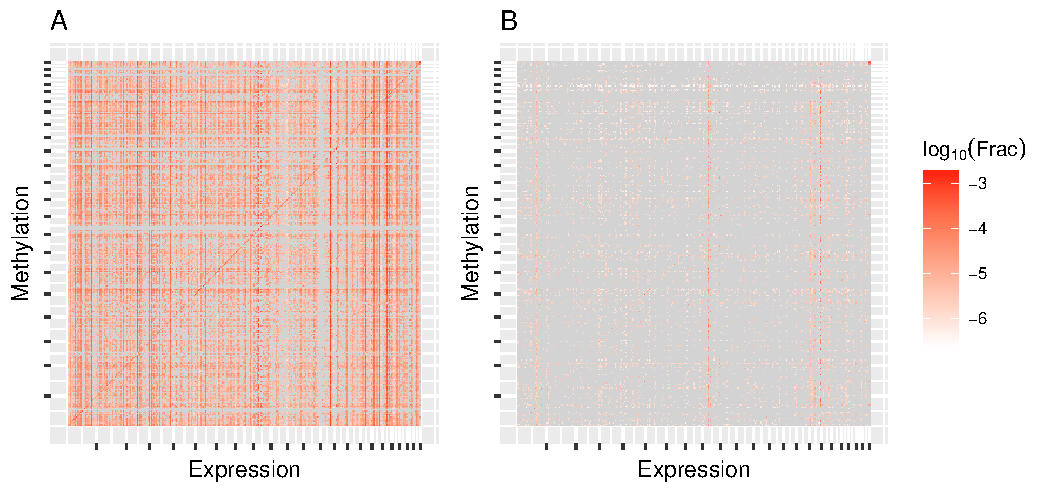
\includegraphics[scale = 1, keepaspectratio = true]{../figures/eqtm_all_herv_heatmap}  
	\caption{Fraction of CpG-expression probe pairs that were significantly associated sorted into bins according to their genomic locations. Ticks on the axis denote chromosome boundaries. Grey means there were no eQTMs in the given pair of bins. A considers all eQTMs and pairs, while B is limited on the ones whose CpGs and/or expression probes are connected to HERV set 2.}
    \label{fig:global.eqtm.heatmap}
\end{figure}

The pairs of expression and methylation residual values for the eQTMs with the best and worst p-values for cis and trans each, are shown in figure \ref{fig:best.worst.eqtm.scatter}. 
%TODO write caption
\begin{figure}[tb]
	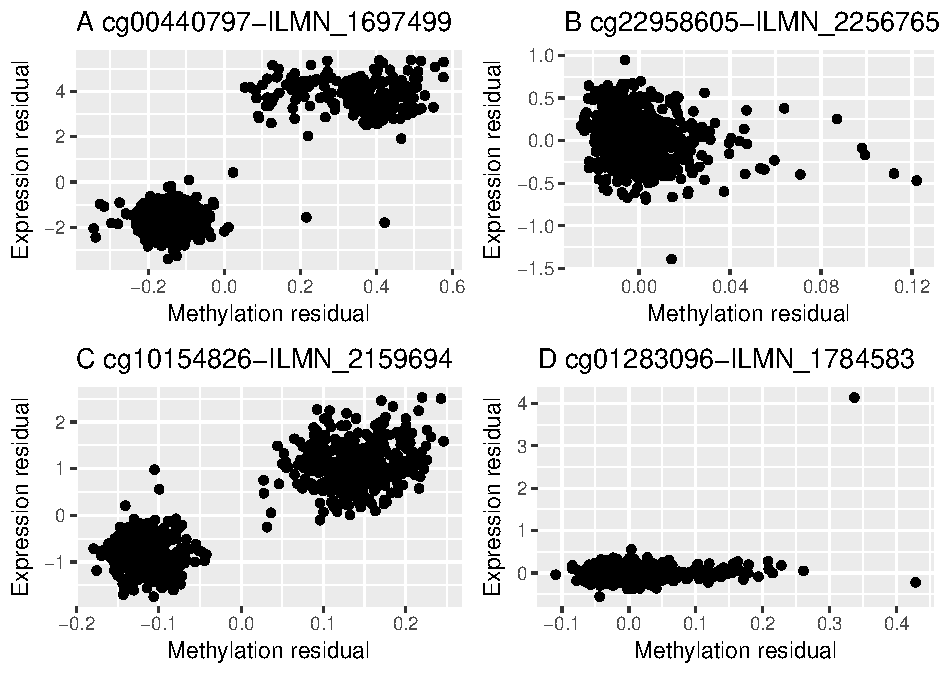
\includegraphics[scale = 1, keepaspectratio = true]{../figures/best_worst_eqtm_scatter.pdf}  
	\caption{}
    \label{fig:best.worst.eqtm.scatter}
\end{figure}

HERV S2 contains 311 CpG sites and 420 expression probes, that were present in cis-eQTMs. A total of 738 cis-eQTMs are related to the set. 33 of these are associations between one of 33 CpG sites and one of 14 expression probes that are both  within a HERV element. 

Considering trans-eQTMs, 1109 significantly associated CpGs lie within HERV S2 and 5422 expression probes overlapping a HERV element are part of a trans-eQTM. In total 15085 trans-eQTMs are related to HERV S2.

The fraction of potential HERV related eQTMs that were significant is shown in figure\ref{fig:global.eqtm.heatmap}B. Due to low number of significant pairs compared to the 90000 cells in the graph it was only sparsely filled. No preference for cis-eQTM could be seen. 

A GO biological process enrichment was performed on the 1316 genes that the expression probes found in HERV S2 related eQTMs are annotated to. All gene that were part of an eQTM were used as background. After correction for multiple testing no GO terms were found to be significantly enriched. 

\section{meQTLs}
\label{Results:meQTLs}
The number of cis- and trans-meQTLs in the obtained data set was already elaborated on in chapter \ref{Data:meQTL}. Therefore, in this chapter the focus is laid on the meQTLs that are related to HERV S2.

There is a total of 360048 meQTLs, whose CpG-site lies within a HERV element. They are made up by 1915 unique CpGs and 286289 SNPs. This means each of these CpG-sites is associated with 188 SNPs on average, which is slightly higher than the average of 157.91 for CpGs in the total set of meQTLs. The CpG, that is part of most meQTLs, cg07143125, is associated with 579 SNPs. 

When considering meQTLs, whose SNP lies within HERV S2, there are 983664 significant CpG-SNP pairs. These consist of 229819 different SNPs and 52951 CpGs. On average each of these SNPs is associated with 4.28 CpG-sites. 

In total there are 1301127 meQTLs, that are related to HERV S2. They are made up of 53167 different CpGs and 483019 SNPs

The fractions of potential SNP-CpG pairs that were significantly associated with respect to their genomic locations are shown in figure \ref{fig:global.meqtl.heatmap}A. Subfigure B shows the same analysis for the subset of meQTLs that were just described. The Fractions of significantly enriched pairs are very similar. The high values along the diagonal show, that there is a strong preference for cis-interactions in both sets. 

\begin{figure}[tb]
	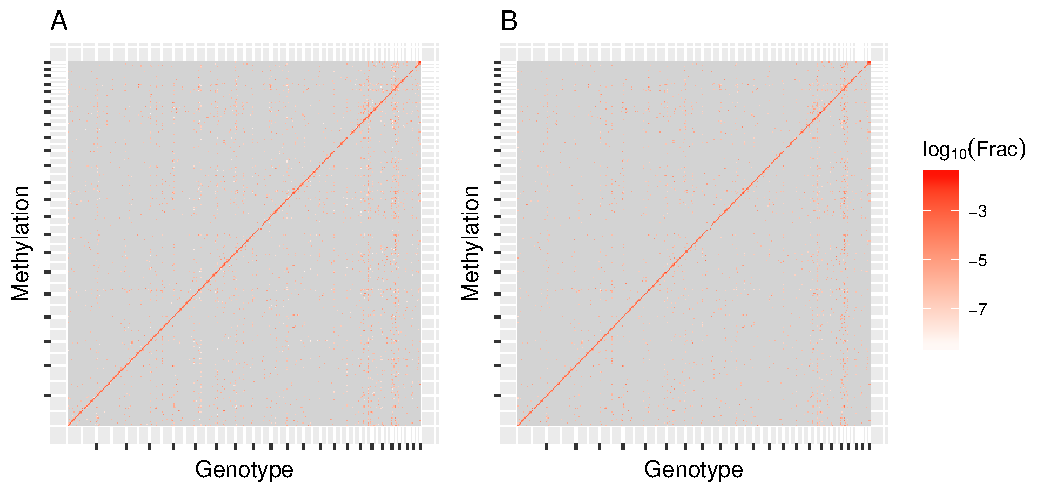
\includegraphics[scale = 1, keepaspectratio = true]{../figures/meqtl_all_herv_heatmap}  
	\caption{Fraction of SNP-CpG pairs that were significantly associated sorted into bins according to their genomic locations. Ticks on the axis denote chromosome boundaries. Grey means there were no eQTMs in the given pair of bins. A considers all meQTLs and pairs, while B is limited on the ones whose CpGs and/or SNPs are related to HERV set 2.}
    \label{fig:global.meqtl.heatmap}
\end{figure}

When limiting the analysis to meQTLs, that represent associations between different chromosomes, what we defined trans-meQTLs, a total of 64852 significant pairs between 2681 CpGs and 34957 SNPs remain. Of these meQTLs, 23463 have their CpGs within HERV S2. They consists of 155 different CpGs and 18825 SNPs. Analogously for 45175 pairs their 19192 SNPs are located within HERV S2 and associated with 2655 different CpGs.

A GO biological process enrichment was performed on the 5128 genes, that contained at least one of the 53167 CpGs that were part of an HERV related meQTL. The significantly enriched terms are shown in table \ref{tab:hervS2.meqtl.enrichment}

\begin{table}[h!]
  \begin{center}
  \resizebox{\textwidth}{!}{
    \pgfplotstabletypeset[
    col sep=tab, 
    header=true,    
	columns={Term ID, Term, p, fdr},
	columns/Term ID/.style={column type=l,string type},
	columns/Term/.style={column type=l,string type},
	every head row/.style={before row=\hline, after row=\hline},
	every last row/.style={after row=\hline}]
    {../tables/hervS2.meqtl.enrichment.tsv}}
  \end{center}        
	\caption{Significantly enriched GO biological process terms among genes containing CpG-sites participating in HERV S2 related meQTLs.}
	\label{tab:hervS2.meqtl.enrichment}
\end{table}

\section{HERV related regulatory networks}
\label{Results:HERV related regulatory networks}
In the following chapter I will present the results of the GGM analysis on HERV related multiomics data. First, I will describe the data sets that were generated according to the two methods described in section \ref{Methods:Data collection}. Next I will give a general overview over the GGMs that were calculated using BDgraph and describe several measures that I used to identify interesting networks. Finally, I will show some of these interesting networks and analyze some of their structures in detail.

\subsection{Data collection}
\label{Results:Data collection}
In the following "entity" describes one of a CpG site, a SNP, a gene or an expression probe.
%SNP seed approach

Filtering the SNPs that were part of at least five trans-meQTLs for relation to elements in HERV S2 resulted in 1885 seed-SNPs. These were consequently used to generate 1883 data sets for GGM calculation accordingly to the criteria defined in \ref{Methods:Data collection}. These sets contained between 13 and 727 entities. The exact size and composition of the biggest (A) and smallest (B) sets is shown in figure \ref{fig:ggm.data.entity.bar}.

In general the biggest groups of entities were CpGs, genes and probes neighboring CpGs and transcription factors. The number genes and probes around the SNP was rather consistent. 1103 of the data sets were enriched with shortest path genes derived from protein-protein interactions. The length of these paths was between 1 and 8. 

For the selection of the CpG based approach, there were 148 CpGs that were part of an trans-meQTL and laid within HERV S2. 103 of these CpGs produced data sets, that contained all demanded types of entities. However, the inclusion criterion of all other CpGs associated to the best associated SNP to any seed CpG lead to some duplicated sets, when the additional CpGs were seed-CpGs themselves. These sets were merged, as their data matrices were identical, which left 100 data sets. 

93 of these started from a single seed CpG, while 4 sets contained two seed CpGs, two sets three and one set four. 

In total there were between 5 and 914 entities per data set. The number and composition of entities in the ten data sets with most (C) and least (D) entities is shown in figure \ref{fig:ggm.data.entity.bar}.

The distribution of different types of entities was similar to the data sets constructed starting from HERV related SNPs. A total of 34 data sets contained shortest path genes of a length between 1 and 10.

%TODO change color scheme
\begin{figure}[tb]
	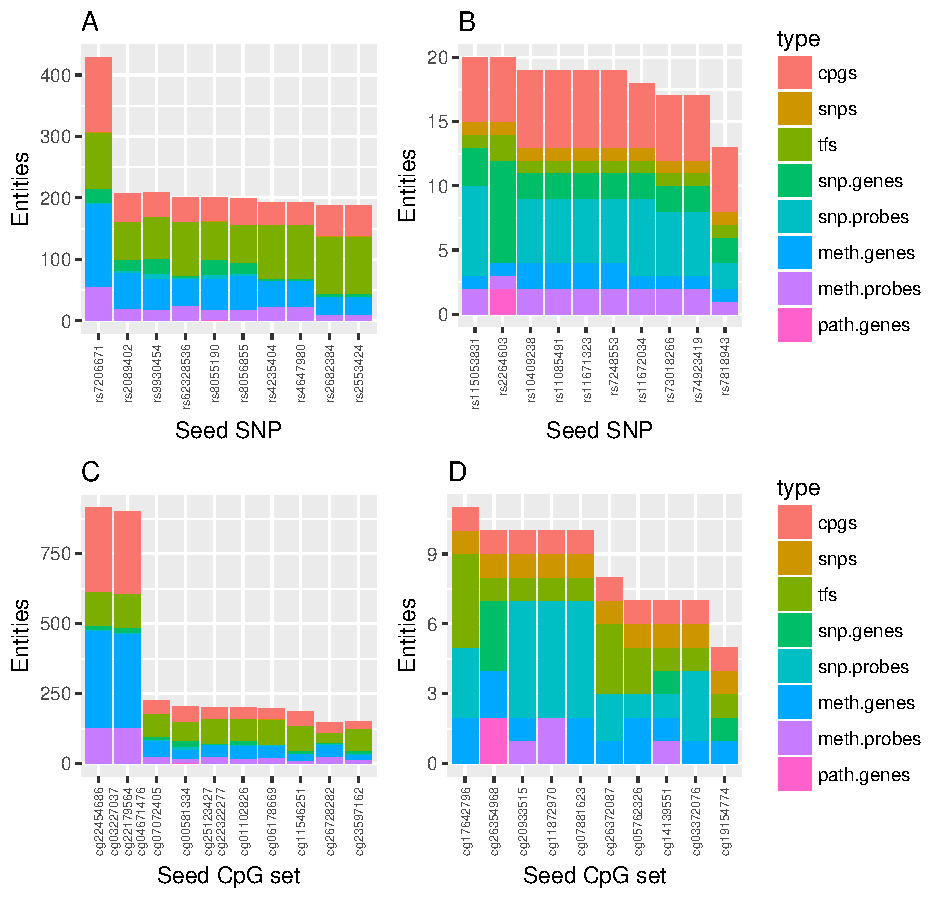
\includegraphics[scale = 1, keepaspectratio = true]{../figures/hervS2_ggm_data_entity_bar}  
	\caption{Size and composition of biggest (left) and smallest (right) GGM data sets. The upper row are sets seeded in HERV-SNPs, while the lower row is seeded in HERV-CpGs. In few cases genes were included as SNP or CpG neighboring gene as well as transcription factor. These genes are displayed as the former.}
    \label{fig:ggm.data.entity.bar}
\end{figure}


\subsection{General networks overview}
\label{Results:General networks overview}
The following section will give a short overview over GGMs calculated as described in section \ref{Methods:GGM calculation and filtering}. 

xxx of the 1883 data sets generated from HERV related SNPs remained after filtering. The restricted networks consisted of between xx and xxx nodes. The actual sizes and compositions of the biggest (A) and smallest networks can be seen in figure \ref{fig:ggm.cc.nodes.bar}.

The networks contained between xx and xxxx edges. 

After filtering the 100 networks seeded in HERV-CpGs, 37 networks remained. The restricted networks contained between 914 and 23 nodes. Their sizes and compositions are shown in figure \ref{fig:ggm.cc.nodes.bar}C.

\begin{figure}[tb]
	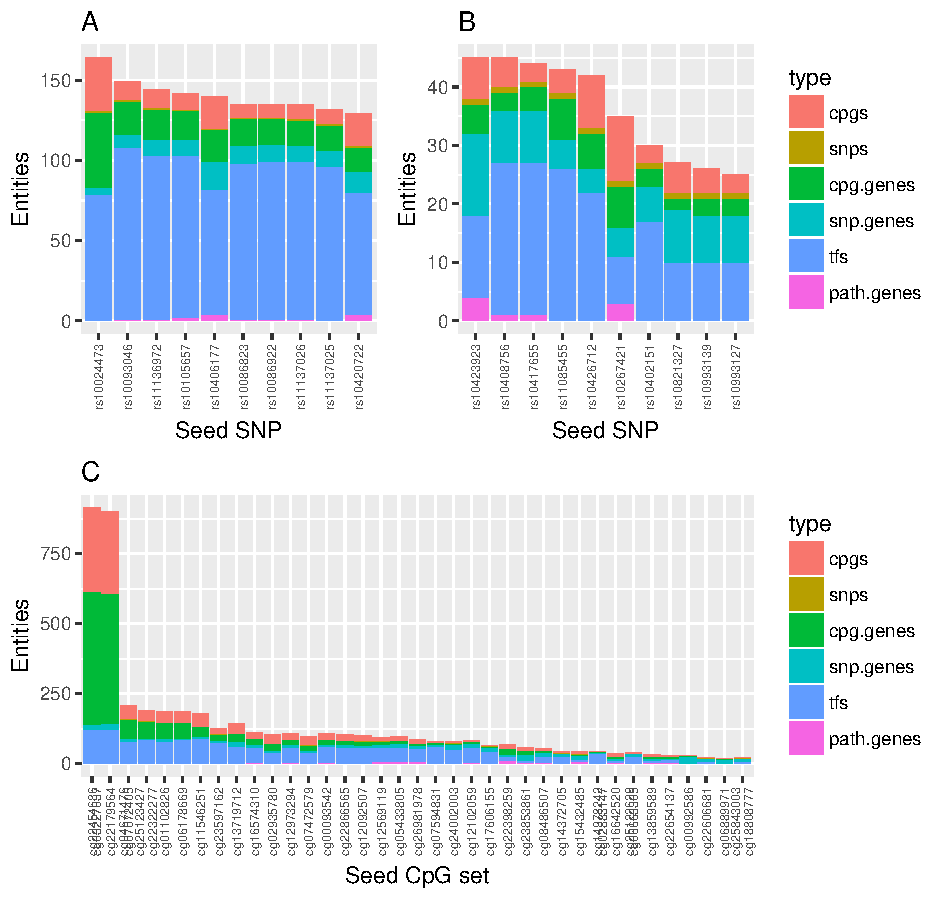
\includegraphics[scale = 1, keepaspectratio = true]{../figures/hervS2_ggm_cc_nodes_bar}  
	\caption{Number and composition of biggest (left) and smallest (right) GGM data sets. The upper row are sets seeded in HERV-SNPs, while the lower row is seeded in HERV-CpGs. In few cases genes were included as SNP or CpG neighboring gene as well as transcription factor. These genes are displayed as the former.}
    \label{fig:ggm.cc.nodes.bar}
\end{figure}

%TODO calculate and add graph measures
\subsection{Example networks}
\label{Results:Example networks}




\newpage
\chapter{Discussion}
\label{Discussion}

\section{HERV region features}
\label{Discussion:HERV region features}

Genotypes, expression levels and methylation levels were measured with microarray based methods. This means no global, unbiased analysis is possible. Therefore, the absence of measurements for many HERV elements is not sufficient to infer e.g. the lack of expression activity. The design of these arrays is not only based on prior knowledge and an assessment of the interest of each probe, but also sequence properties. For example the data sheet for the HumanHT-12 v3 Expression BeadChip\cite{HumanHT} mentions as parameters for the probe design among others the lack of similarity to other genes and the absence of highly repeated sequence in the genome. As a result it is to be expected, that HERVs, which are considered repeats after all, are covered sparsely. 

\subsection{Expression}
\label{Discussion:Expression}
The number of available expression measurements within HERV elements was lower than expected, if the probes were randomly distributed. This is explained by the mentioned limitations in probe design, as well as the focus on annotated genes. This was supported by the result, that while over 60\% of all probes on the HumanHT-12 v3 Expression BeadChip are annotated to a gene, less than one fourth of the probes overlapping with HERVs belong to a gene.

The enrichment of genes associated with the GO term "defense response" among them might conform with prior findings. Products encoded by HERVs have been found to play a role in host protection against viral infection\cite{Malfavon-Borja2015}.

The distribution of expression values of HERV associated probes shows, that there certainly is expression activity within HERV elements. While the variance of expression values tends to be lower than on the entire data set, it is still enough for differential analyses. 

\subsection{Methylation}
\label{Discussion:Methylation}
The amount of probes measuring CpG-sites with HERV elements also was lower than would be expected, if probes were randomly distributed. This is expected to be due to probe design instead actual CpG occurrence. However an actual calculation of CpG density in HERV elements was not performed. 

The high average of methylation level of HERV CpGs is in line with observations, that HERV LTRs tend to be methylated in order to silence their promoter activity\cite{Smith2013}.

\subsection{Genotypes}
\label{Discussion:Genotypes}
The availability of genotype measurements was an exception, as the fraction of SNPs within HERV elements was slightly higher than the fraction of the genome covered by HERVs. This might be represent an actual higher density of common variants in HERV elements, as they are known to be highly degenerated and experience almost no evolutionary pressure pressure\cite{10.1146/annurev.genom.7.080505.115700}.

\section{eQTLs}
\label{Discussion:eQTLs}
We identified a high number of significant cis- as well as trans-eQTLs in the data set. Nevertheless, pairs of SNPs and expression probes are a lot more likely to be associated when they are in cis. This agrees with previous findings\cite{}.

Interestingly a far higher percentage of probes taking part in cis-eQTLs at about 85\% is annotated to a gene, compared to probes in trans-eQTLs at 44\%. %TODO why?
 
The distributions of expression residuals for the significant eQTLs with worst p-values, shown in figure \ref{fig:best.worst.eqtl.boxplot}B and D, might hint towards setting a stricter cutoff. However, matrixEQTL works with continuous dosages instead of the discrete variants shown in the figure. This might disguise a more palpable association of the variant on the expression levels.

About 65\% of the cis-eQTLs identified by Schramm et al\cite{Schramm2014} were reproduced in this analysis. Considering that only a subset of the data was used and they methods as well as thresholds for the calculation of significant eQTLs were different, this is a good overlap. 

The number of HERV related eQTLs shows that there certainly is some variation within HERV elements. Especially the high number of expression probes significantly associated with SNPs that lie within HERV elements shows the wide reaching effects. However, eQTLs do not grant insight into the underlying mechanisms. 

This high number of probes and subsequently also genes might be the reason, that the GO enrichment on genes being part of HERV related eQTLs produced no significant results. xx\% of the genes that were part of any eQTL were also found in the filtered set.
\section{eQTMs}
\label{Discussion:eQTMs}


\section{meQTLs}
\label{Discussion:meQTLs}
\begin{itemize}
\item 
\item go-enrichment: neuro related -> associated with neurodegenerative diseases\cite{Mortelmans2016}, like schizophrenia\cite{10.3389/fpsyt.2015.00183}
\end{itemize}

\section{Regulatory networks}
\label{Discussion:Regulatory networks}
\begin{itemize}
\item data collection not perfect
\item example networks:
\begin{itemize}
\item cg25843003|cg18808777: direct cpg-snp edge/only con through each other: maybe true path members not  present, multiple step path weaker than strong direct association, direct cpg-(trans-)snp gene edge is surprising
\end{itemize}
\item add priors to guide analysis 
\end{itemize}


\newpage
\chapter{Conclusion and Outlook}
\label{Conclusion and Outlook}

\newpage
\listoffigures
\listoftables

\bibliography{mybib}{}
\bibliographystyle{unsrtMod}

\end{document}